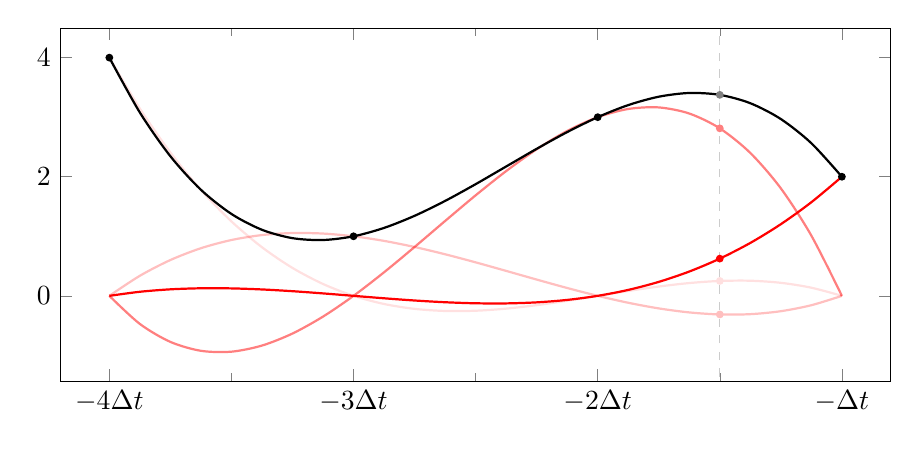
\begin{tikzpicture}
  \begin{axis}[xmin=-4.2, xmax=-0.8, width=\columnwidth, height=0.5\columnwidth,
      xtick={-4, -3, -2, -1},
      minor x tick num={1},
      xticklabels={$-4\Delta t$, $-3\Delta t$, $-2\Delta t$, $-\Delta t$}
  ]


% Unweighted basis polynomials
  %\draw[dashed, opacity=0.2] (axis cs:-1.2,-10) -- (axis cs:-1.2,10) {};

  %\addplot[red, opacity=1.00, smooth, domain=-4:-1]{1/6*(2+x)*(3+x)*(4+x)};
  %\addplot[red, opacity=0.50, smooth, domain=-4:-1]{1/2*(-1-x)*(3+x)*(4+x)};
  %\addplot[red, opacity=0.25, smooth, domain=-4:-1]{1/2*(-2-x)*(-1-x)*(4+x)};
  %\addplot[red, opacity=0.12, smooth, domain=-4:-1]{1/6*(-3-x)*(-2-x)*(-1-x)};

  %\node[fill, red,            circle, inner sep=1.0pt] (p1) at (axis cs:-1.2,0.672) {};
  %\node[fill, red!50!white,   circle, inner sep=1.0pt] (p2) at (axis cs:-1.2,0.504) {};
  %\node[fill, red!25!white,   circle, inner sep=1.0pt] (p3) at (axis cs:-1.2,-0.224) {};
  %\node[fill, red!12.5!white, circle, inner sep=1.0pt] (p4) at (axis cs:-1.2,0.048) {};

% Weighted basis polynomials
  \draw[dashed, opacity=0.2] (axis cs:-1.5,-10) -- (axis cs:-1.5,10) {};

  \addplot[thick, red, opacity=1.00, smooth, domain=-4:-1]{1/3*(2+x)*(3+x)*(4+x)};
  \addplot[thick, red, opacity=0.50, smooth, domain=-4:-1]{3/2*(-1-x)*(3+x)*(4+ x)};
  \addplot[thick, red, opacity=0.25, smooth, domain=-4:-1]{1/2*(-2-x)*(-1-x)*(4+x)};
  \addplot[thick, red, opacity=0.12, smooth, domain=-4:-1]{2/3*(-3-x)*(-2-x)*(-1-x)};

  \node[fill, red,            circle, inner sep=1.0pt] (p1) at (axis cs:-1.5,0.625) {};
  \node[fill, red!50!white,   circle, inner sep=1.0pt] (p2) at (axis cs:-1.5,2.8125) {};
  \node[fill, red!25!white,   circle, inner sep=1.0pt] (p3) at (axis cs:-1.5,-0.3125) {};
  \node[fill, red!12.5!white, circle, inner sep=1.0pt] (p4) at (axis cs:-1.5,0.25) {};

% Actual interpolated function
  \addplot[thick, smooth, domain=-4:-1]{2/3*(-3-x)*(-2-x)*(-1-x) + 1/2*(-2-x)*(-1-x)*(4+x) + 3/2*(-1-x)*(3+x)*(4+x) + 1/3*(2+x)*(3+x)*(4+x)};

  \node [fill, gray, opacity=1.00, circle, inner sep=1.0pt] (pol) at (axis cs:-1.5,3.375) {};
  %\node [fill, gray, opacity=1.00, circle, inner sep=1.0pt] (pol) at (axis cs:-1.2,2.824) {};

  \node [fill, black, circle, inner sep=1.0pt] (x1) at (axis cs:-1,2) {};
  \node [fill, black, circle, inner sep=1.0pt] (x2) at (axis cs:-2,3) {};
  \node [fill, black, circle, inner sep=1.0pt] (x2) at (axis cs:-3,1) {};
  \node [fill, black, circle, inner sep=1.0pt] (x2) at (axis cs:-4,4) {};

  \end{axis}
\end{tikzpicture}
